\chapter{Motorola SmartConnect}
\label{smart-connect}
In this chapter, we introduce the reader to the domain of the analyzed product.
We aim to detect anomalies in logs produced by software system called SmartConnect by company Motorola Solutions.

We introduce the business perspective of the product which should help the reader gain insight into why the mission critical system would benefit from an anomaly detection tool.
Also, we provide a high level introduction into the software architecture of the solution that is crucial to understanding what anomalies can happen, where logs are created and how to collect them.

\section{Domain Description}

\textit{Two-way radio} (also a push-to-talk, informally a walkie-talkie  \cite{twowayradio}) is an electronic device that enables a group of people to communicate.

A two-way radio works by converting audio signal to radio waves that are transmitted through the air to receivers. On the receiving end, the waves are converted back to audio signal which allows the recipients to hear the original message.
There are two alternatives of what kind of signal is being transmitted through the air - it can be either analogue or digital.
The advantage of radios that support digital signal is that they can transfer various types of data over the channel, not only the audio. On the other hand, analogue transmission has been the standard for audio data transmission for many years.

Two-way radios are using frequencies between 30MHz and 1000MHz \cite{twowayradio}. The interval between 30MHz and 300MHz is referred to as Very High Frequency and the remaining upper part is called Ultra High Frequency \cite{twowayradio}.


\subsection{Motorola SmartConnect}

SmartConnect is a software product by company Motorola Solutions. 
The state of the art Motorola two-way radios \cite{apxp25radio} support automatic switching in favor of the source strongest signal.

The classical way of interconnecting a set of walkie-talkies is through narrowband land mobile radio (LMR) sites.
However, due to specifics of the network, there is many use-cases where a push-to-talk device is out of range of LMR \cite{apxnextslides}. 

% Use cases
There are many different environments where customers of Motorola Solution's operate and it must be made sure that they get the best connectivity possible. 
However, not everywhere LMR coverage is sufficient. 
Indoor areas such as hospitals, offices or schools are usually equipped with high quality WiFi connection which can be exploited instead.
Also, if mobile broadband, for example LTE \cite{dahlman20134g}, is more accessible than LMR, cellular data can be also taken advantage of. And for the least accessible areas, radio may connect to a satellite modem to ensure the customer doesn't lose contact with colleagues.

Motorola products are compliant with Project 25 (P25 for short) which is an LMR standard that is well suited for fast, secure and interoperable connection \cite{project25}.

A radio with SmartConnect support is able to automatically switch to LTE, WiFi, satellite broadband or even wired internet connection ensuring continuity of push-to-talk voice communications in case strength of the LMR signal drops below specified RSSI (received signal strength indication) threshold. 
The radio is able to switch back to LMR when the signal strengthens with no user intervention required \cite{apxnextfactsheet} \cite{businesswireapxnext}.
The structure of a Motorola PTT radio network is schematically explained in Figure~\ref{smart-connect:smart-connect-architecture}.

\begin{figure}[h]
    \centering
    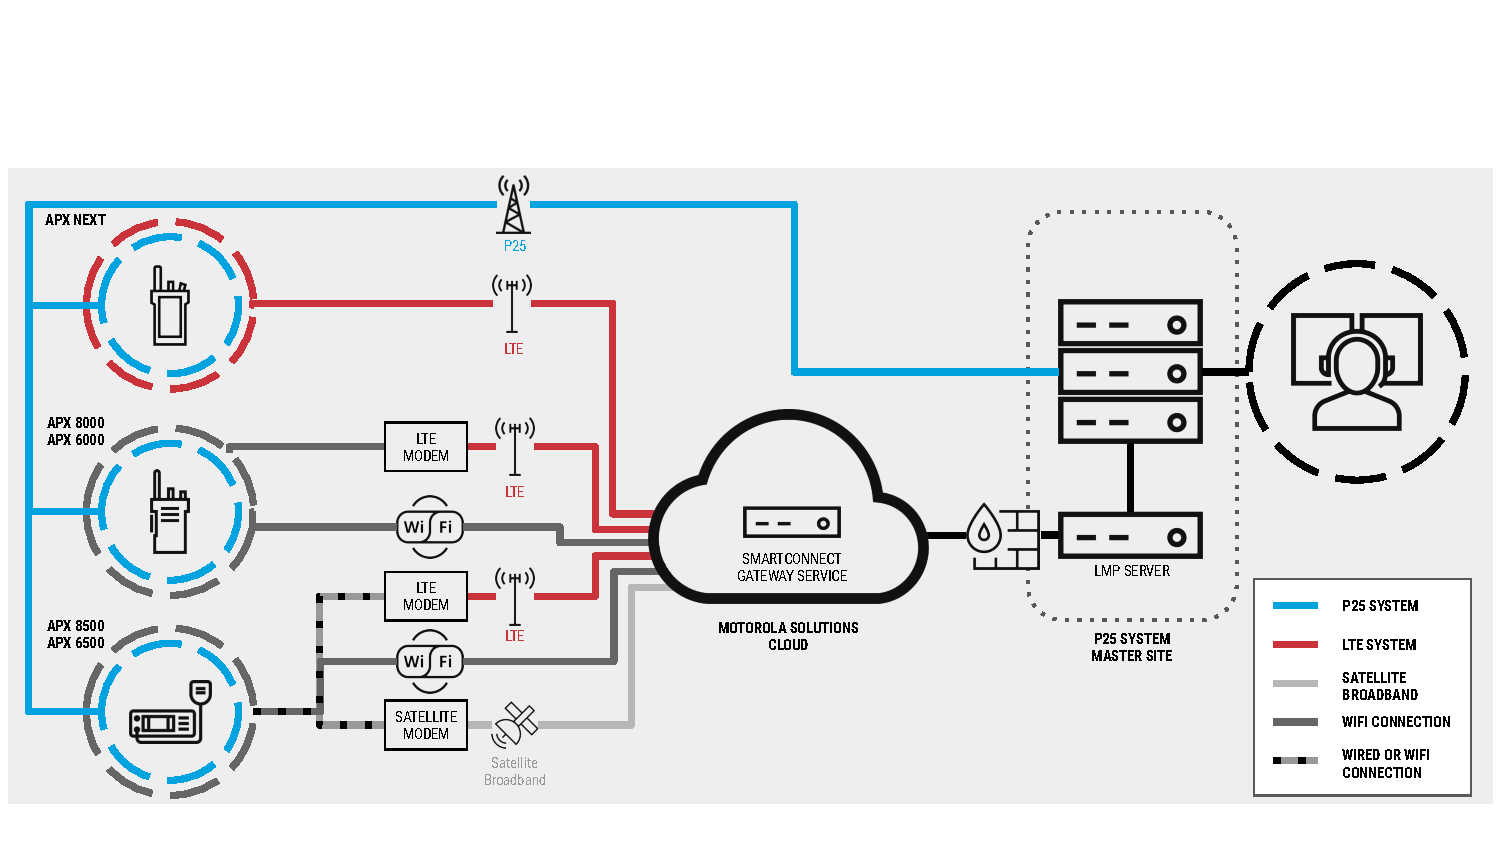
\includegraphics[width=\textwidth]{img/motorola-smart-connect-architecture.pdf}
    \caption{Overview of Motorola two-way radio network showing the various technologies that can be exploited to interconnect push-to-talk radios \cite{apxnextslides}.}
    \label{smart-connect:smart-connect-architecture}
\end{figure}

When a radio utilizes the SmartConnect technology, voice packets are being transferred through the broadband bearer to a cloud-based gateway. This gateway in the cloud connects to the LMR master site. This allows the radios communicating over SmartConnect call back in the LMR system \cite{apxnextslides}.

Therefore, Motorola Solution's SmartConnect helps teams stay connected no matter where they are located by leveraging various means of voice packet transmission.

\section{Software Architecture of SmartConnect}
\label{smart-connect:architecture}

Now let's have a look at the core concepts that form the whole cloud based gateway functionality from the software architecture perspective. 

Having familiarity with the architecture of SmartConnect is important for being able to tackle the anomaly detection problem in an informed way. It gives us a better understanding of what are the weak links that are prone to error about the software.
In this thesis we want to target anomalies based on logs. Knowing the architecture also helps with identifying what parts of the system produce logs that can be collected and extracted information from.

The software follows the \textit{Microservices Architecture} (MSA).
Nadareishvili et al. \cite{nadareishvili2016microservice} define a \textit{microservice} as an independently deployable component of bounded scope that supports interoperability through message-based communication. 

Fowler \cite{fowler2014microservices} understands the microservice architectural style as a way of building a single application by connecting a set of small services. Each of the services runs in its own process and communicates with lightweight mechanisms.

Another attribute of such an architecture is that management of the service is decentralized, therefore it allows for the individual services to be written in various programming languages and use different technologies for storing their data.

A collection of services that communicate together form a \textit{system} \cite{indrasiri2018microservices}.

\subsection{Deployment}

In the analyzed system, the individual services are deployed as Docker\footnote{\url{https://www.docker.com/}} containers in Kubernetes Pods\footnote{\url{https://kubernetes.io/docs/concepts/workloads/pods/}} which are self-standing applications inside of Kubernetes\footnote{\url{https://kubernetes.io/}} clusters.

This approach allows the services to be decoupled as each one resides in its own isolated virtual container.

As described in more detail in Chapter~\ref{data_collection} on Data Collection, the services log each at a different location by default. 
In order to analyze the behaviour of the system holistically, an extra layer for processing logs has to be introduced. SmartConnect, like many others, for this use-case utilizes the Elasticsearch engine that also runs as one of the services in the cluster.

High level view of a Motorola SmartConnect Kubernetes cluster is presented later when discussing the way we deployed our tool for downloading logs from the Elasticsearch service in Figure~\ref{fig:data_collection_elastic}.


\subsection{Elasticsearch}
\label{smart-connect:elastic-search}
Elasticsearch\footnote{\url{https://www.elastic.co/elasticsearch/}} is an open-source, distributed search engine. Gormley and Tong \cite{gormley2015elasticsearch} argue that it can be used for exploring data at unprecedented speed. It is mostly recognized for its exceptional performance on text based data. Operations such as full-text search, structured search and analysis are supported efficiently.
Elasticsearch can also be defined as a NoSQL database since it gathers JSON based \texttt{documents} of a specific \texttt{type} together and multiple \texttt{types} are organized into \texttt{indices}\footnote{\url{https://www.elastic.co/blog/what-is-an-elasticsearch-index}}. 

\subsection{Messaging}
\label{architecture:messaging}
As mentioned earlier, services in an MSA application may be designed in a different way and two services are free to use two dissimilar sets of technologies. That makes the communication within a system more complicated than calling a function - what one would do in a traditional, monolithic architecture.

Two main strategies of passing messages between system's services are \textit{synchronous} and \textit{asynchronous} communication. One of the most common types of synchronous communication is Representational state transfer (REST) \cite{indrasiri2018microservices}.

On the other hand, asynchronous communication promotes autonomy between services as the communicating client does not need to wait for the response. 
For implementation of asynchronous protocols, the concept of a \textit{broker} is introduced. A broker is a centralized entity with high-availability \cite{indrasiri2018microservices}.

In SmartConnect, services are passing values asynchronously. In order to achieve some high-level goal, services form a chain of $1$ or more microservices. Each link of the chain receives an input, processes it and if needed, forwards its output through a broker to another microservice(s) that take(s) this data as input.

For dealing with asynchronous messages, \texttt{RabbitMQ}\footnote{https://rabbitmq.com/documentation.html} brokers are deployed.
\texttt{RabbitMQ} is an open-source publisher/subscriber message broker.

\subsection{Storing Data}
\label{architecture:caching}
In microservices architecture systems, microservices that are immutable and stateless are favoured \cite{indrasiri2018microservices}. 
Therefore, data that the internal state of a microservice comprises of needs to be persisted in storage that is external to memory of a microservice application.

Traditionally, a database is utilized for persisting data externally to the application. However, it is well known that there are major set back when it comes to performance of read/write operations that can be improved by deploying supporting caches \cite{elhardt1984database}.

Performance of the system is fairly crucial as, among others, UDP (user datagram protocol) audio packets of push-to-talk radio calls are being transferred and processed in the system. 
In order to satisfy strict requirements on jitter in the audio signal, a NoSQL data storage Redis\footnote{https://redis.io/} service is running inside of the Kubernetes cluster to serve requests for the stored data rapidly.
